\chapter*{\label{ref-007}Werken in Amsterdam}

Na Engeland heb ik in Amsterdam gewerkt; intern in het Wilhelmina gasthuis. Ik zat in die periode veel in het Vondelpark, ik vond dit een leuke tijd maar ik moet er nu niet meer aan denken om in Amsterdam te wonen. 

In het Wilhelmina gasthuis werkte ik als huishoudkundige, ik gaf leiding aan de meisjes die daar werkten in de huishouding. 

Ze noemden me dan Juf, zo hoorde dat. Ik dacht toen; dit werk wil ik niet blijven doen tot aan mijn pensioen.

\begin{figure}[h!]
    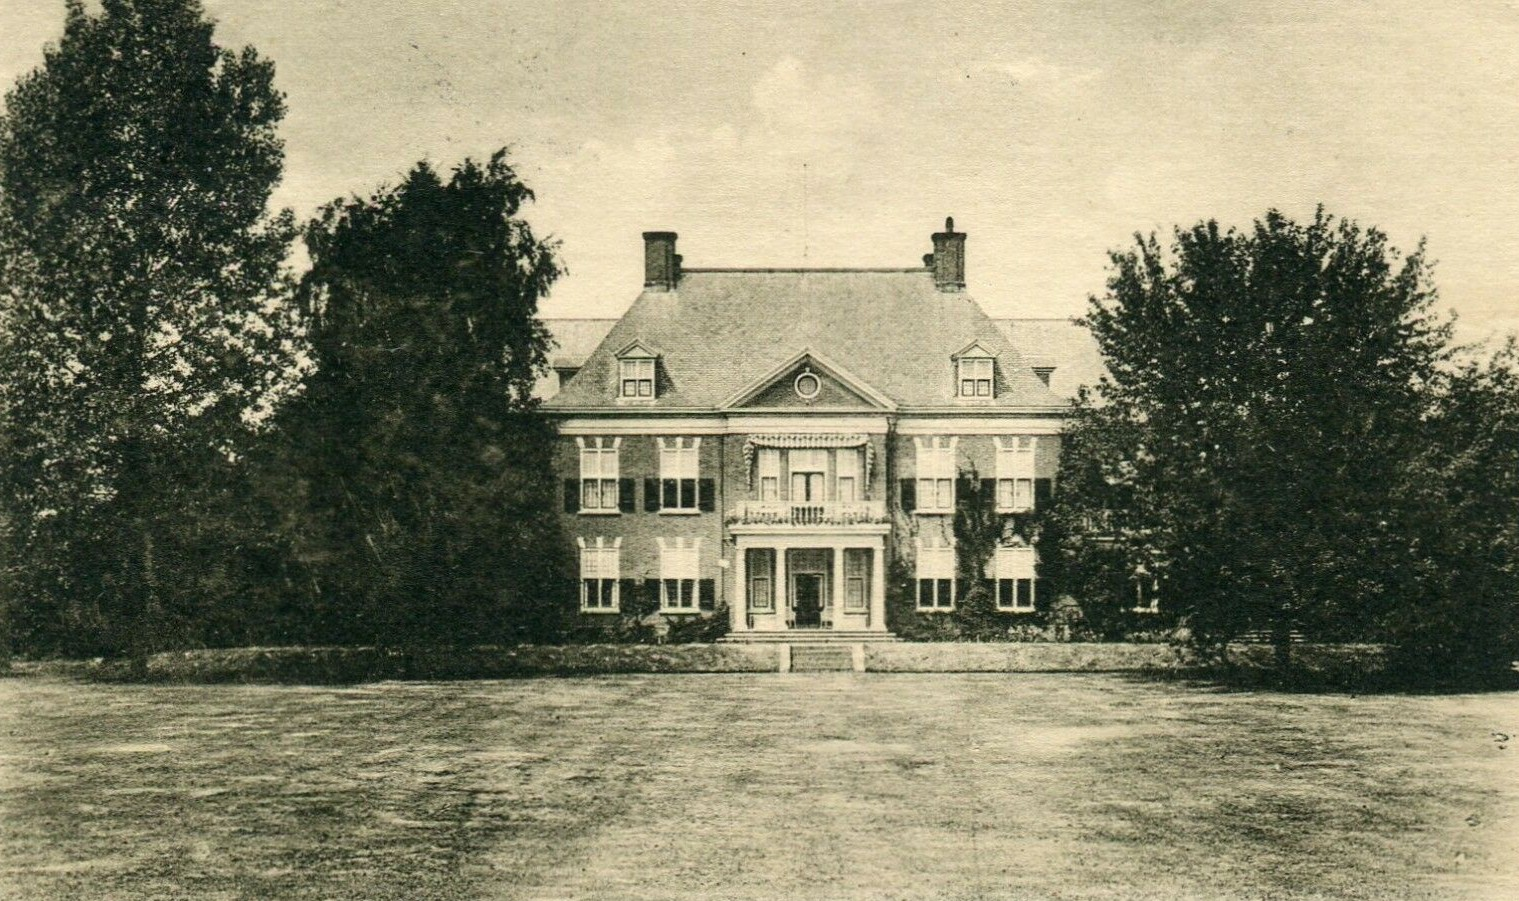
\includegraphics[width=\textwidth]{image35}
    \caption{Huis ter wege.}
\end{figure}

Daarna ben ik begonnen bij de Kinderbescherming in huis ter Wege (in het dorp Huis ter Heide). Eerst had ik hier de leiding in de keuken (koken voor 50 mensen) en daarna heb ik daar als jeugdleidster gewerkt. 

% \begin{figure}[h]
%     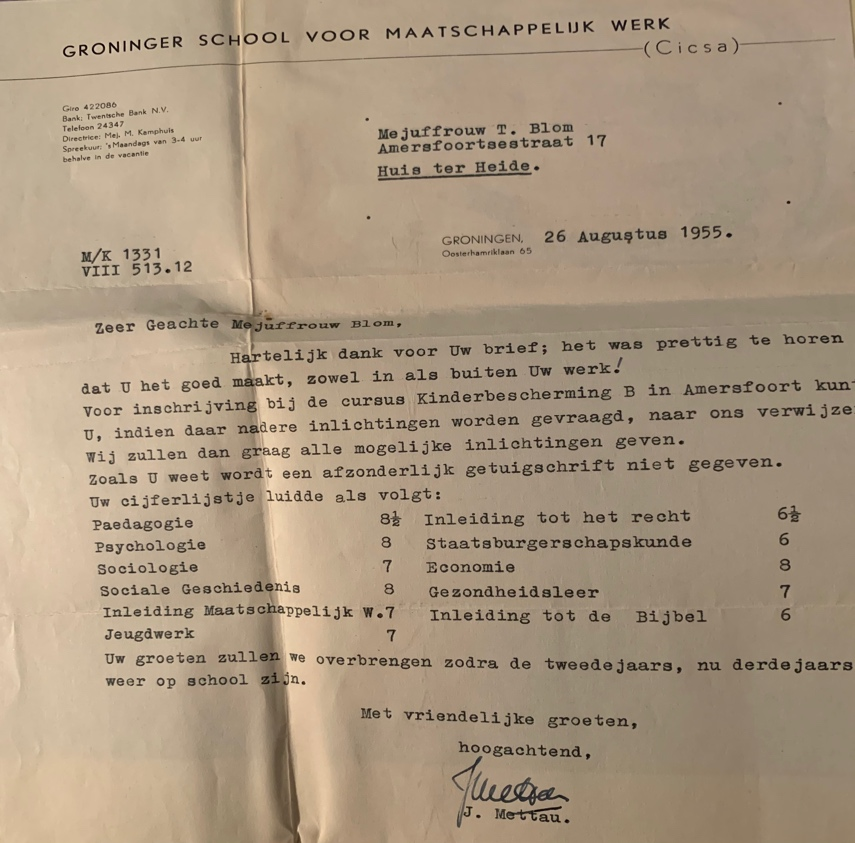
\includegraphics[width=\textwidth]{image33}
%     \caption{Cijferlijst van de Groninger school voor maatschappelijk werk.}
% \end{figure}

Intern heb ik hier een opleiding voor gedaan zodat ik met deze jeugd kon werken. In Groningen kreeg ik dan les, dit moest in mijn vrije tijd. Hier kreeg ik ook lessen in de psychologie, dat vond ik heel interessant. 

\begin{figure}[h]
    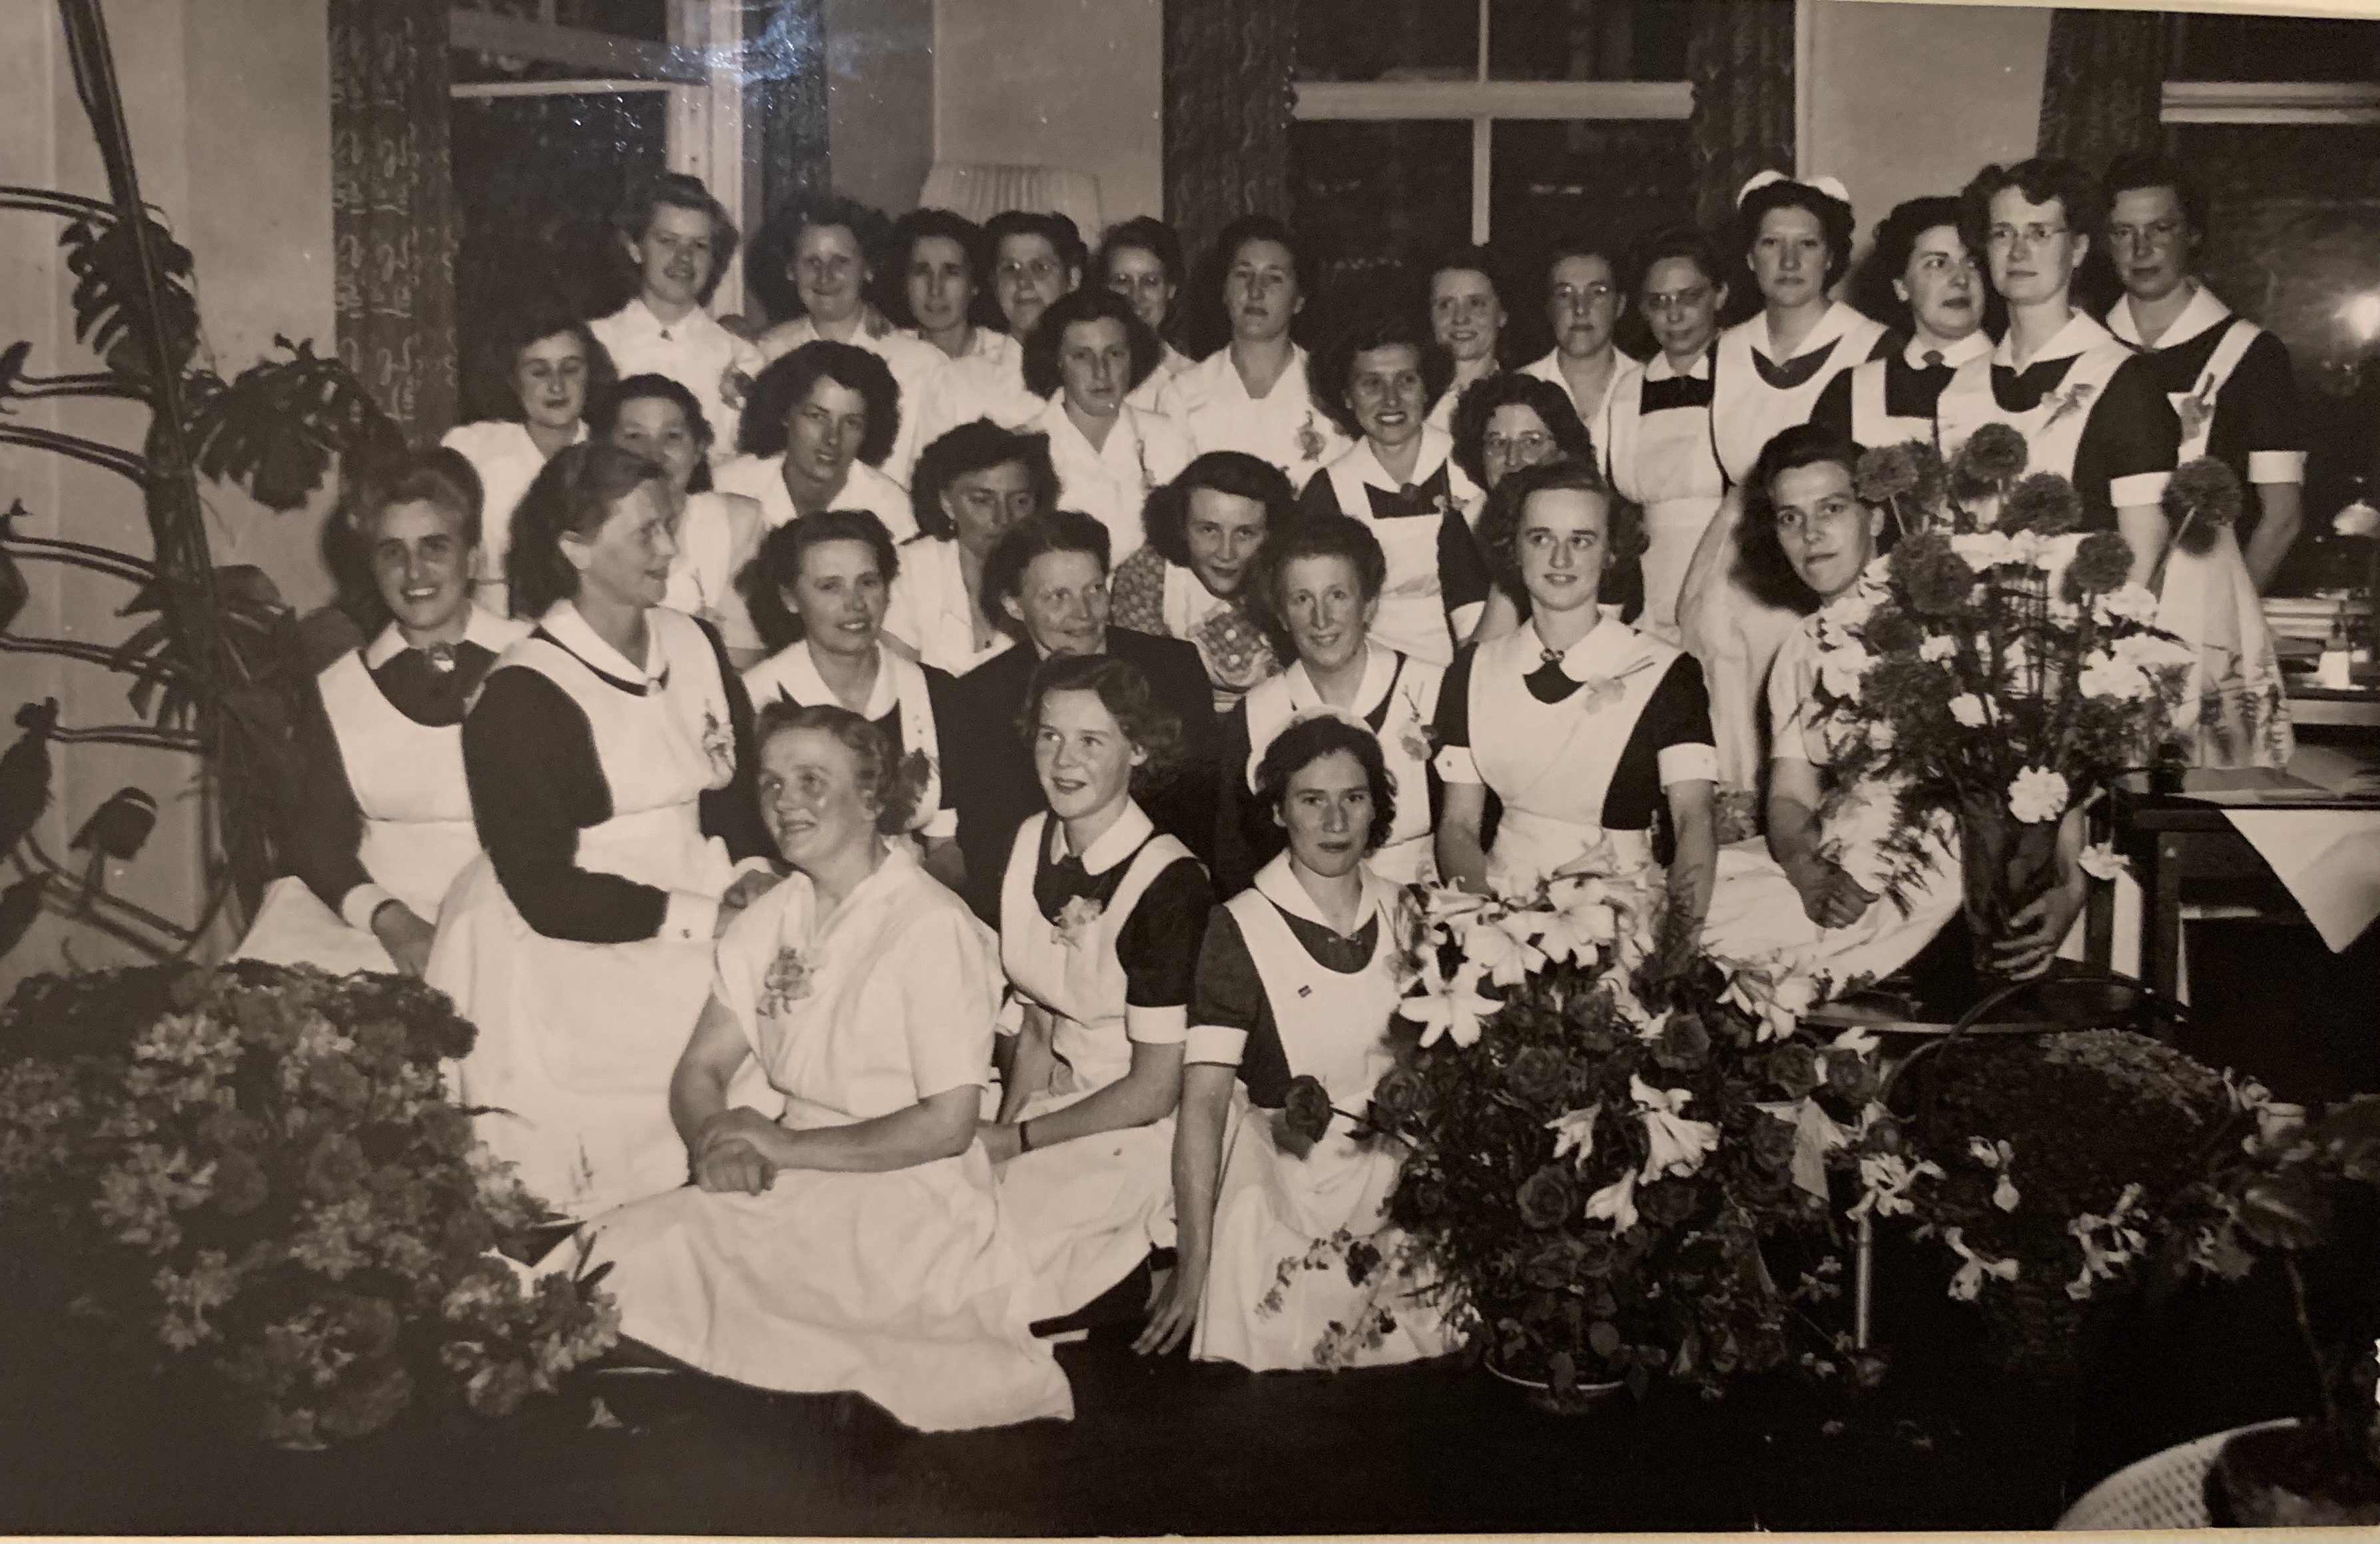
\includegraphics[width=\textwidth]{image32}
    \caption{De dames van de Kinderbescherming.}
\end{figure}

Totdat ik ging trouwen heb ik hier gewerkt, ongeveer van mijn 22\textsuperscript{e} tot mijn 28/29\textsuperscript{e}. In Huis ter Heide had je \'{e}\'{e}n jeugdleidster per afdeling van 12 kinderen, en je zat intern maar je had wel je eigen kamer.

\begin{figure}[h]
    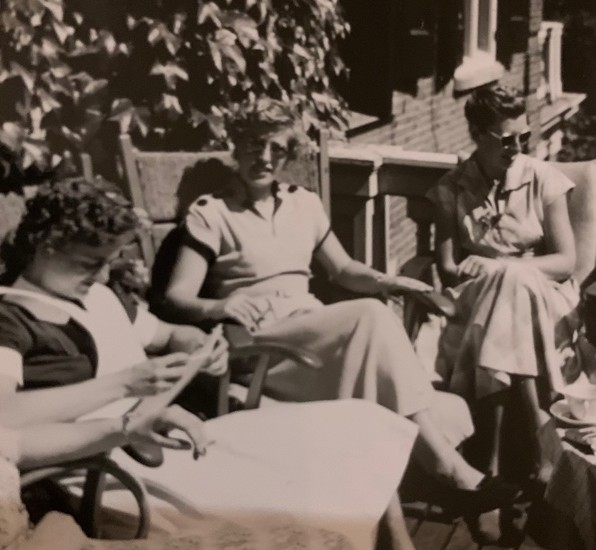
\includegraphics[width=\textwidth]{image34}
    \caption{De staf van Ter Wege drinkt koffie.}
\end{figure}

Ik begon daar met werken in de keuken, een paar meisjes hielpen mij dan. Daarna kreeg ik steeds meer taken, waaronder kookles geven het maken van de planning en het rooster. 

Ik ben ook nog een periode waarnemend directrice geweest. Ik vond het leuk werk, vooral het werken met kinderen. 

\begin{figure}[]
    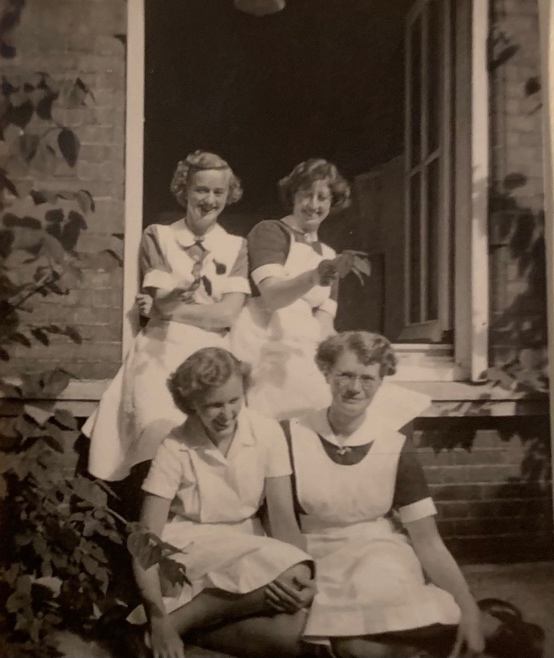
\includegraphics[width=\textwidth]{image31}
    \caption{Op het Wilhelmina Gasthuis.}
\end{figure}

Deze kinderen werden vrijwillig geplaatst door het maatschappelijk werk of de school en ze knapten vaak flink op van hun verblijf bij ons. Als de kinderen binnenkwamen moesten ze vaak huilen, ik zei dan; als jullie over 3 maanden vertrekken dan moeten jullie weer huilen en dat was ook altijd zo. 

De kinderen waren 10 tot 12 jaar. Er was eens een meisje uit Egmond aan zee wat na haar verblijf langs kwam op bezoek, dit vonden we heel erg leuk. 

